\begin{figure}[p]
\centering
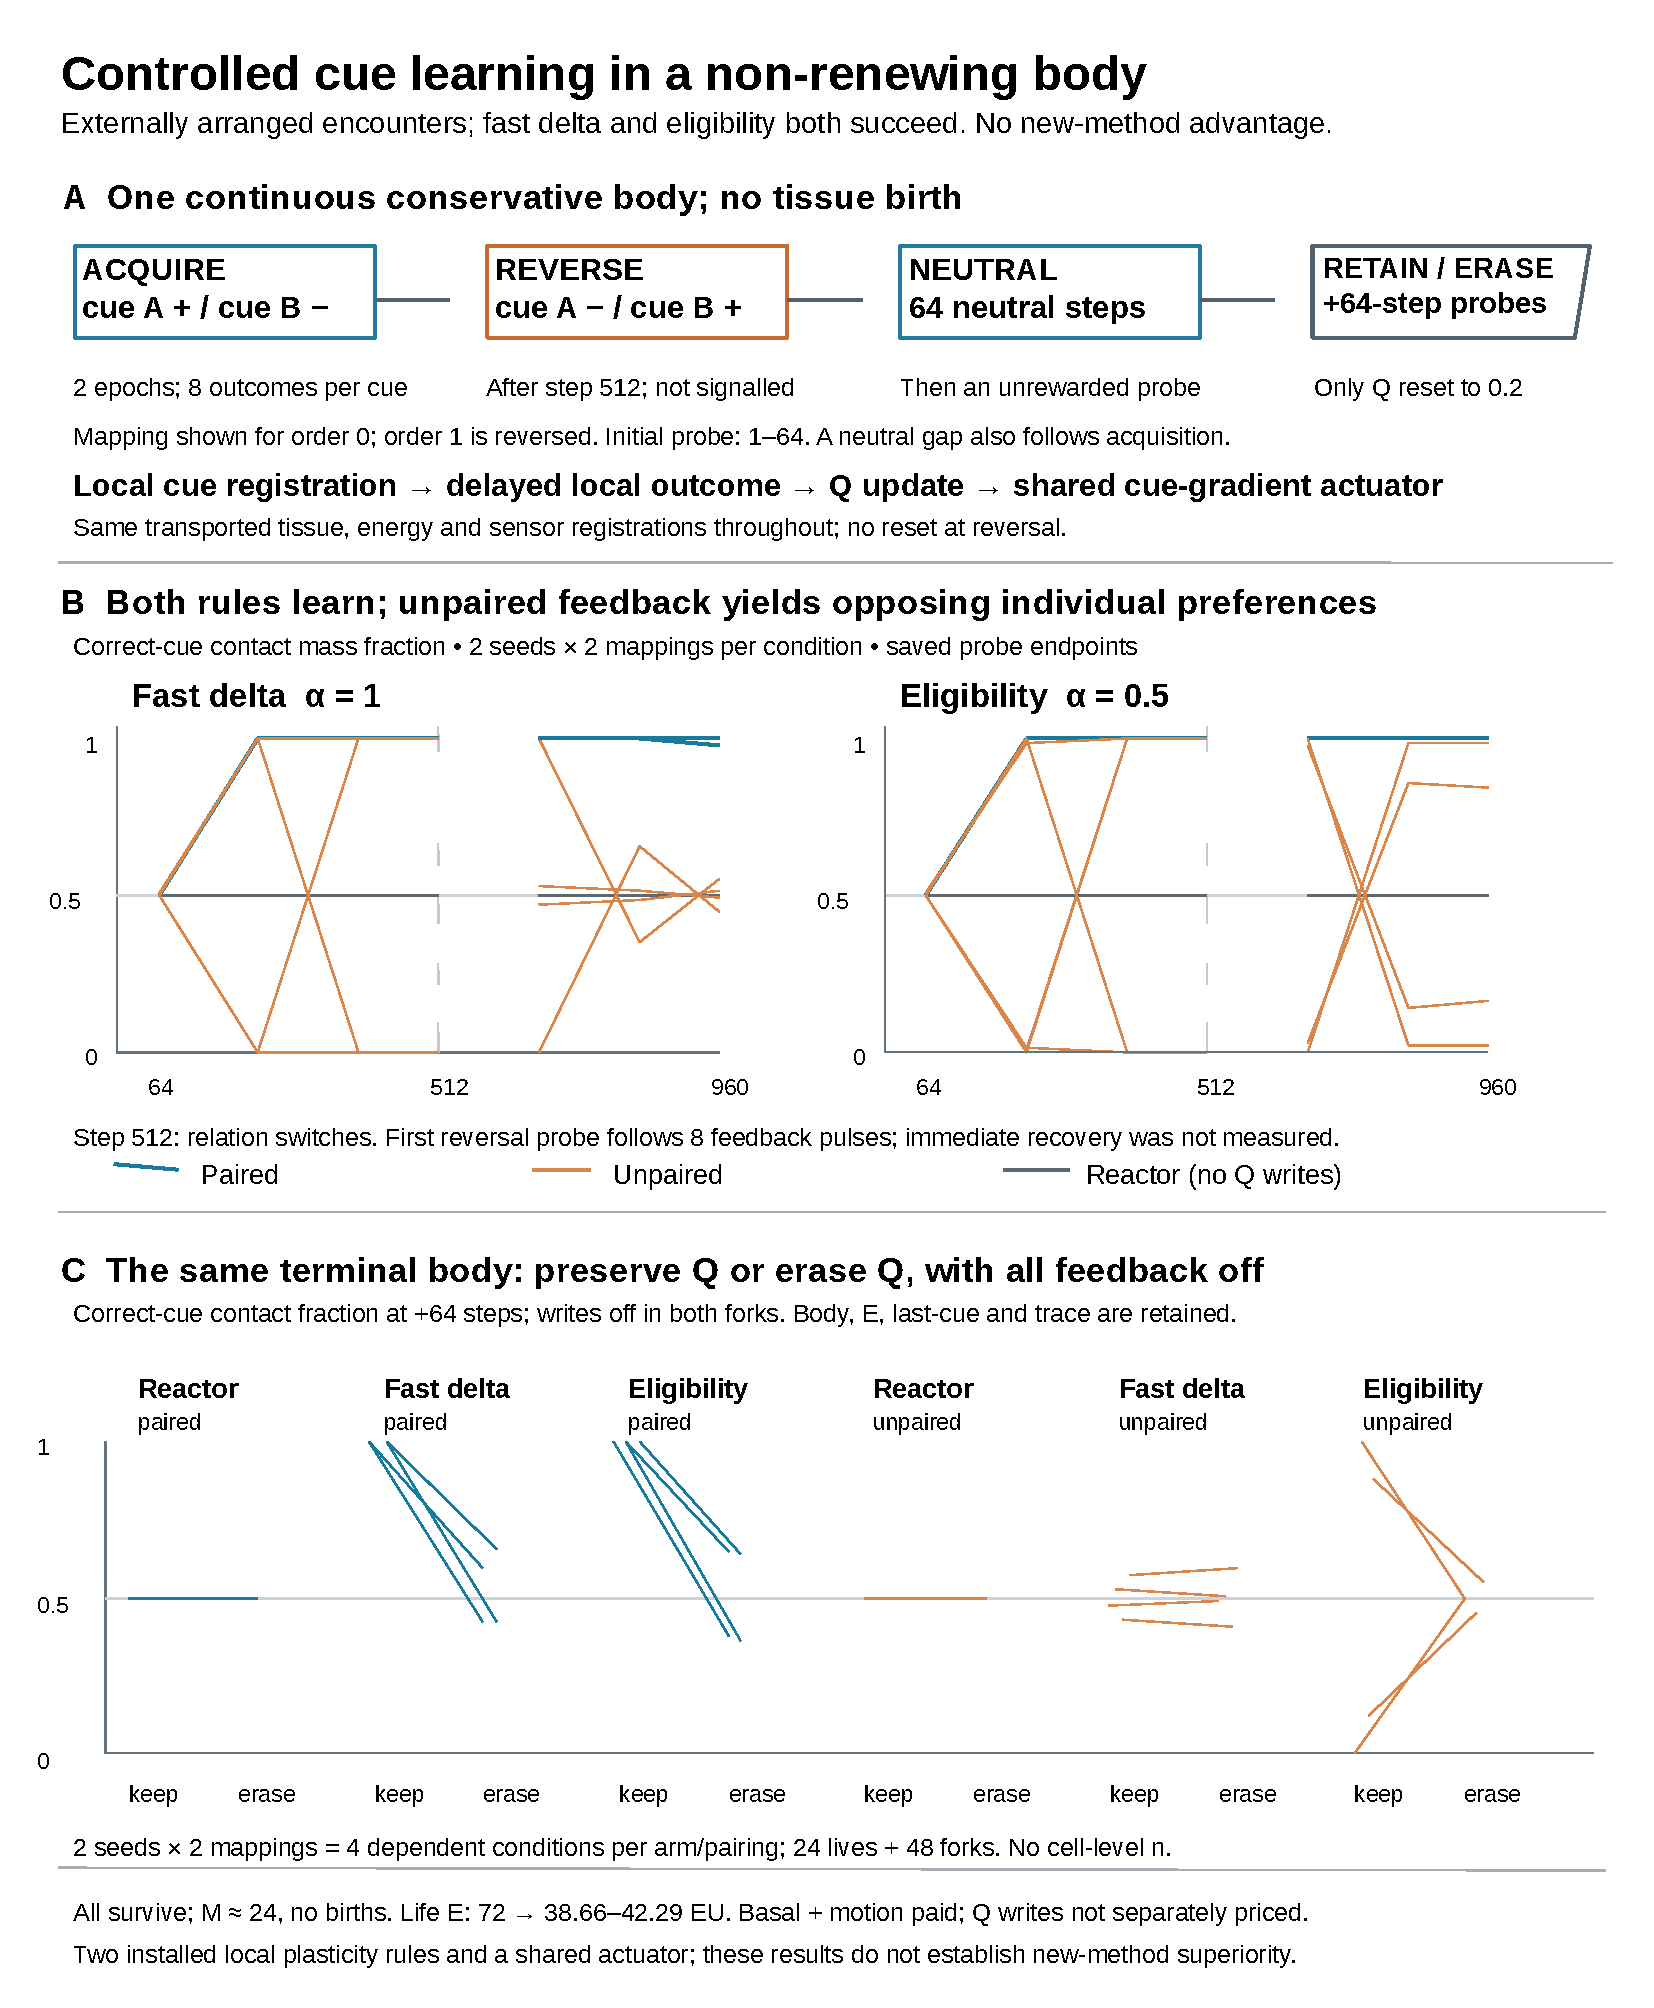
\includegraphics[width=\linewidth,height=.76\textheight,keepaspectratio]{work/longform_v047/figures/lifetime_learning_v0474/lifetime_learning.pdf}
\caption{\textbf{Controlled cue learning in a non-renewing body.}
\textbf{a}, Externally arranged encounters on one continuing conservative body, without tissue birth. \textbf{b}, Two installed update rules, recent-feedback (fast delta) and eligibility, acquire and reverse cue preference in a continuing transported body. Four related seed--mapping paths per condition retain the individual outcomes: the unpaired mean near one half hides opposing preferences. \textbf{c}, Matched terminal freeze/erase forks change only the initial stored cue values, preserving body, energy and sensory registrations at branching. The first reversal probe follows eight new feedback pulses. All paths survive in this no-birth host, while movement and basal costs reduce available energy. Neither update rule establishes a new-method advantage. Values are actual probe contact fractions; repeated phases and terminal forks are not independent histories.}
\label{fig:lifetime-learning}
\end{figure}
